\documentclass[10pt,letterpaper]{article}
\usepackage[margin=0.9in]{geometry}
\usepackage{amsmath,graphicx,booktabs,float,caption}
\captionsetup{font=small,labelfont=bf}
\makeatletter\renewcommand\section{\@startsection{section}{1}{0pt}{-8pt}{3pt}{\normalfont\large\bfseries}}\makeatother
\setlength{\parskip}{3pt}
\title{\vspace{-1.2cm}Your model A with a time integration in place of the one-second kick}
\author{Addendum to the parameter scans at $R=14.3$ Gpc}
\date{September 26, 2026}
\begin{document}
\maketitle\vspace{-0.8cm}

\section{What changed}
Your sheet computes each source's velocity as the Hubble velocity plus a single kick, $S=J+Q\,\Delta t$ with $\Delta t=1$~s. Here that kick is replaced by an integration of the equations of motion over the whole expansion history, in your geometry and with your density profile, sine factor and final formula. The CoE sits at the origin, Earth at $(D,0)$ today, and source $P$ at Earth $+\,R(\cos\theta,\sin\theta)$ today with $\theta=\ell$. Table~\ref{tab:vars} lists the quantities in your notation. The one deliberate departure is Newton's constant: the integration uses the SI value, whereas your sheet uses $1000$ times that value. Because a physical $G$ and a physical time span now set the size of the effect, the mass is quoted as $M/M_{\rm crit}$ as well as in kilograms.

\begin{table}[H]\centering\small
\caption{Variables, in your notation. $M_{\rm crit}$ uses $H_0=70$ km\,s$^{-1}$\,Mpc$^{-1}$.}\label{tab:vars}
\begin{tabular}{lll}\toprule
Symbol & Meaning & Value or range\\\midrule
$R$ & distance from Earth to the source shell & 14.3 Gpc ($4.4127\times10^{23}$ km)\\
$D$ & distance from the CoE to Earth today & $D/R$ scanned over 1.05--10\\
$L$ & scale length of the $e^{-r/L}$ density profile & $L/D$ scanned over 0.02--3\\
$M$ & mass inside radius $D$ & $M/M_{\rm crit}$ scanned over $10^{-3}$--10\\
Amp, $\varphi$ & amplitude and phase of your sine term BA & $|{\rm Amp}|\le0.15$, $0\le\varphi<2\pi$\\
$\theta$, $\ell_0$ & source angle, optional axis offset & $\theta=\ell$, or $\theta=\ell-\ell_0$\\
$k$, $t_0$ & your expansion rate and the present time & $2.18\times10^{-18}$ s$^{-1}$, $t_0=1/k$\\
$t_i$ & start time of the integration & $0.01\,t_0$ (also 0.001 and 0.05)\\
$G$ & Newton's constant & $6.674\times10^{-11}$ SI (your sheet: $\times1000$)\\
$M_{\rm crit}$ & critical mass inside $D$, $\tfrac{4}{3}\pi\rho_cD^3$ & $H_0^2D^3/2G$\\\bottomrule
\end{tabular}\end{table}

\section{Integration}
Without gravity the flow is homologous, $v=r/t$, so every point moves as
\begin{equation}\label{eq:flow}
\mathbf{x}_0(t)=\mathbf{q}\,t/t_0,\qquad \dot{\mathbf{x}}_0=\mathbf{q}/t_0,
\end{equation}
where $\mathbf{q}$ is its position today. Earth and each source start on this flow at $t_i$, $\mathbf{x}(t_i)=\mathbf{q}\,t_i/t_0$ and $\dot{\mathbf{x}}(t_i)=\mathbf{q}/t_0$, and are then moved by the enclosed mass,
\begin{equation}\label{eq:eom}
\ddot{\mathbf{x}}=-\,\frac{G\,M(<|\mathbf{x}|,t)}{|\mathbf{x}|^{3}}\,\mathbf{x},\qquad
M(<r,t)=M\,\frac{f\!\left(r/L(t)\right)}{f\!\left(D/L_0\right)},\qquad f(u)=1-e^{-u}\left(1+u+\tfrac12u^2\right),
\end{equation}
which is the enclosed mass of an $e^{-r/L}$ density normalised so that $M$ lies inside $D$. The requested main case lets the profile expand with the flow, $L(t)=L_0\,t/t_0$; the check case holds it fixed, $L=L_0$. Your amplification factor becomes the ratio of the source's velocity relative to Earth today, with and without gravity,
\begin{equation}\label{eq:AF}
{\rm AF}(\theta)=\frac{\left|\dot{\mathbf{x}}_P(t_0)-\dot{\mathbf{x}}_E(t_0)\right|}{kR},\qquad
A(\theta)=\left[1-{\rm Amp}\,\sin(\theta+\varphi)\right]{\rm AF}(\theta),
\end{equation}
and in units of $D$ and $t_0$ the strength of gravity is the single number
\begin{equation}\label{eq:mu}
\mu=\frac{G M t_0^2}{D^3},\qquad \frac{M}{M_{\rm crit}}=2\mu\left(\frac{k}{H_0}\right)^{2}=1.847\,\mu .
\end{equation}
Positions today drift slightly under gravity, so Eq.~(\ref{eq:AF}) compares at $t_0$ without forcing the sources back onto your geometry. In the shot variant the starting points are instead adjusted iteratively, $\mathbf{q}\to\mathbf{q}+[\mathbf{q}_{\rm target}-\mathbf{x}(t_0)]$, until $\mathbf{x}(t_0)$ matches your geometry. The integrator is fourth-order Runge--Kutta in $\ln t$, checked against DOP853 at a relative tolerance of $10^{-11}$. Any configuration in which a particle turns around and falls back before today is excluded as unphysical. The amplitude and phase of the sine are fitted by exact linear least squares at every trial of $D/R$, $L/D$ and $M$.

\section{Results}
The comoving main case is ill-posed. With $M$ fixed inside the comoving $D$, the density falls as $t^{-3}$ while the flow's $H^2=1/t^2$, so the density parameter grows toward early times as $t_0/t$. The integrated kick grows as $\int dt/t^2$ and is set almost entirely at the start. The fitted mass is therefore proportional to $t_i$ (Table~\ref{tab:sens}), and the result is simply one impulse delivered at $t_i$ to a scaled copy of your geometry. That is why its best fit reproduces the impulse fit's $D/R$, $L/D$, amplitude, phase and $R^2$ (Table~\ref{tab:fit}). The fixed profile is well-posed, because early on every particle sits inside the core, where the pull grows only linearly with radius, and the integral converges. We take it as the working integrated model.

In the fixed-profile model the best fit prefers a much more compact mass, $L/D\approx0.07$, and $M/M_{\rm crit}\approx0.02$. The one-parameter profiles (Fig.~\ref{fig:prof}) and the map (Fig.~\ref{fig:map}) show a long, flat ridge in which $L/D$ and $M$ trade off against each other, so $M$ is poorly constrained along it. Landing the final positions exactly on your geometry moves the optimum along that ridge to $L/D=0.165$ and $M/M_{\rm crit}=0.15$, at the same $R^2$. That is the physical range you expected and close to your $L/D=0.18$. Your literal mass is $10^{12}$ times critical and recollapses almost immediately, so that row cannot be computed. With your geometry and sine values and only $M$ re-fitted, the model reaches the $R^2$ given in Table~\ref{tab:fit}.

The integration does not change the shape of your model A. The best integrated and impulse curves are indistinguishable (Fig.~\ref{fig:best}), and their harmonic amplitudes agree to about $0.001$ (Table~\ref{tab:harm}). Both carry the same deficit against $A_F$ in the second and third harmonics, which is the part of $A_F$ your model does not yet reproduce. What changes is the geometry that produces that shape. The integrated AF on its own is almost purely a second harmonic, and the sine term supplies essentially all of the first harmonic. The $\ell_0\approx13^\circ$ axis offset improves the integrated fit by the same amount it improved the impulse fit.

\begin{table}[H]\centering\footnotesize\setlength{\tabcolsep}{3.2pt}
\caption{Best fits at $R=14.3$ Gpc, impulse (previous addendum) versus integrated. ``Fixed'' is the fixed-profile integration from $t_i=0.01\,t_0$ compared at $t_0$; ``shot'' lands the final positions on your geometry; ``comoving'' is the expanding profile. $R^2$ is against the 71 Migkas points or against $A_F$.}\label{tab:fit}
\begin{tabular}{lccccccccccc}\toprule
Case & $D/R$ & $L/D$ & $D$ [Gpc] & $L$ [Gpc] & $M$ [kg] & $M/M_{\rm crit}$ & Amp & $\varphi$ & $\ell_0$ & $R^2_{\rm Migkas}$ & $R^2_{A_F}$\\\midrule
Impulse, best vs Migkas & 2.26 & 0.295 & 32.3 & 9.51 & $2.48\times10^{69}$ & $6.5\times10^{13}$ & $-0.046$ & 0.21 & -- & 0.759 & 0.833\\
Impulse, with $\ell_0$ & 2.45 & 0.297 & 35.0 & 10.4 & $3.54\times10^{69}$ & $7.3\times10^{13}$ & $-0.042$ & 0.45 & 13.0$^\circ$ & 0.897 & 0.981\\
Impulse, your values & 5 & 0.18 & 71.5 & 12.9 & $4.44\times10^{68}$ & $1.1\times10^{12}$ & $-0.06$ & 0.35 & -- & 0.266 & 0.295\\\midrule
Fixed, best vs Migkas & 2.71 & 0.072 & 38.7 & 2.79 & $1.44\times10^{54}$ & 0.022 & $-0.052$ & 0.51 & -- & 0.755 & 0.829\\
Fixed, with $\ell_0$ & 2.90 & 0.070 & 41.5 & 2.92 & $1.94\times10^{54}$ & 0.024 & $-0.051$ & 0.75 & 13.2$^\circ$ & 0.894 & 0.979\\
Fixed, best vs $A_F$ & 2.48 & 0.072 & 35.5 & 2.57 & $1.10\times10^{54}$ & 0.022 & $-0.052$ & 0.50 & -- & 0.754 & 0.829\\
Fixed, vs $A_F$ with $\ell_0$ & 2.73 & 0.071 & 39.0 & 2.77 & $1.62\times10^{54}$ & 0.024 & $-0.051$ & 0.73 & 13.1$^\circ$ & 0.894 & 0.980\\
Fixed and shot, best vs Migkas & 2.47 & 0.165 & 35.3 & 5.81 & $7.36\times10^{54}$ & 0.148 & $-0.049$ & 0.38 & -- & 0.757 & 0.831\\
Comoving, $t_i=0.01\,t_0$ & 2.22 & 0.294 & 31.7 & 9.30 & $5.1\times10^{52}$ & 0.0014 & $-0.046$ & 0.18 & -- & 0.760 & 0.834\\
Comoving, $t_i=0.001\,t_0$ & 2.21 & 0.294 & 31.7 & 9.30 & $5.1\times10^{51}$ & 0.00014 & $-0.046$ & 0.18 & -- & 0.760 & 0.834\\
Fixed, your values, $M$ re-fitted & 5 & 0.18 & 71.5 & 12.9 & $3.01\times10^{55}$ & 0.073 & $-0.06$ & 0.35 & -- & 0.653 & 0.717\\
Fixed, your values and your $M$ & 5 & 0.18 & 71.5 & 12.9 & $4.44\times10^{68}$ & $1.1\times10^{12}$ & $-0.06$ & 0.35 & -- & \multicolumn{2}{c}{recollapses}\\\bottomrule
\end{tabular}\end{table}

\begin{table}[H]\centering\footnotesize\setlength{\tabcolsep}{4pt}
\caption{Sensitivity of the fixed-profile best fit to the start time and to shooting, and of the comoving fit to the start time. ``Change in AF'' is the largest relative change over all angles at the $t_i=0.01\,t_0$ best-fit parameters; the refit columns re-optimise $D/R$, $L/D$, $M$, Amp and $\varphi$. The integration error is below $10^{-12}$ for the fixed profile (800 steps) and for the comoving profile (20000 steps).}\label{tab:sens}
\begin{tabular}{lccccccc}\toprule
Variant & \shortstack{Change\\in AF} & \shortstack{$R^2$ at same\\parameters} & \shortstack{Refit\\$D/R$} & \shortstack{Refit\\$L/D$} & \shortstack{Refit\\$M/M_{\rm crit}$} & \shortstack{Refit\\$R^2_{\rm Migkas}$} & \shortstack{Final position\\error / $D$}\\\midrule
Fixed, $t_i=0.05\,t_0$ & $5.1\times10^{-3}$ & 0.7526 & 2.63 & 0.089 & 0.0297 & 0.7552 & 0.065\\
Fixed, $t_i=0.01\,t_0$ & reference & 0.7546 & 2.71 & 0.072 & 0.0219 & 0.7546 & 0.065\\
Fixed, $t_i=0.001\,t_0$ & $2.8\times10^{-4}$ & 0.7545 & 2.72 & 0.071 & 0.0213 & 0.7545 & 0.065\\
Fixed and shot, $t_i=0.01\,t_0$ & $5.7\times10^{-2}$ & 0.5474 & 2.47 & 0.165 & 0.148 & 0.7569 & $5\times10^{-10}$\\
Comoving, $t_i=0.01\,t_0$ & -- & -- & 2.22 & 0.294 & 0.00142 & 0.7601 & --\\
Comoving, $t_i=0.001\,t_0$ & -- & -- & 2.21 & 0.294 & 0.00014 & 0.7601 & --\\\bottomrule
\end{tabular}\end{table}

\begin{table}[H]\centering\footnotesize
\caption{Harmonic amplitudes of $A(\theta)$ over the full circle (Fourier coefficients $m=1,2,3$ and the root-sum-square of $m\ge4$). The last two rows are AF before the sine factor is applied. The best integrated and impulse model A agree with an $R^2$ of 0.9997 against each other, with an rms difference of $1.0\times10^{-3}$.}\label{tab:harm}
\begin{tabular}{lcccc}\toprule
Curve & $m=1$ & $m=2$ & $m=3$ & $m\ge4$\\\midrule
$A_F$ & 0.0525 & 0.0734 & 0.0320 & 0\\
Your model A, impulse best fit & 0.0530 & 0.0659 & 0.0235 & 0.0071\\
Your model A, integrated fixed best fit & 0.0528 & 0.0659 & 0.0222 & 0.0070\\
Your model A, integrated fixed and shot & 0.0529 & 0.0659 & 0.0228 & 0.0070\\
Your model A, integrated comoving & 0.0531 & 0.0659 & 0.0238 & 0.0071\\
AF only, impulse best fit & 0.0200 & 0.0659 & 0.0238 & 0.0072\\
AF only, integrated fixed best fit & 0.0037 & 0.0661 & 0.0231 & 0.0073\\\bottomrule
\end{tabular}\end{table}

\begin{figure}[H]\centering
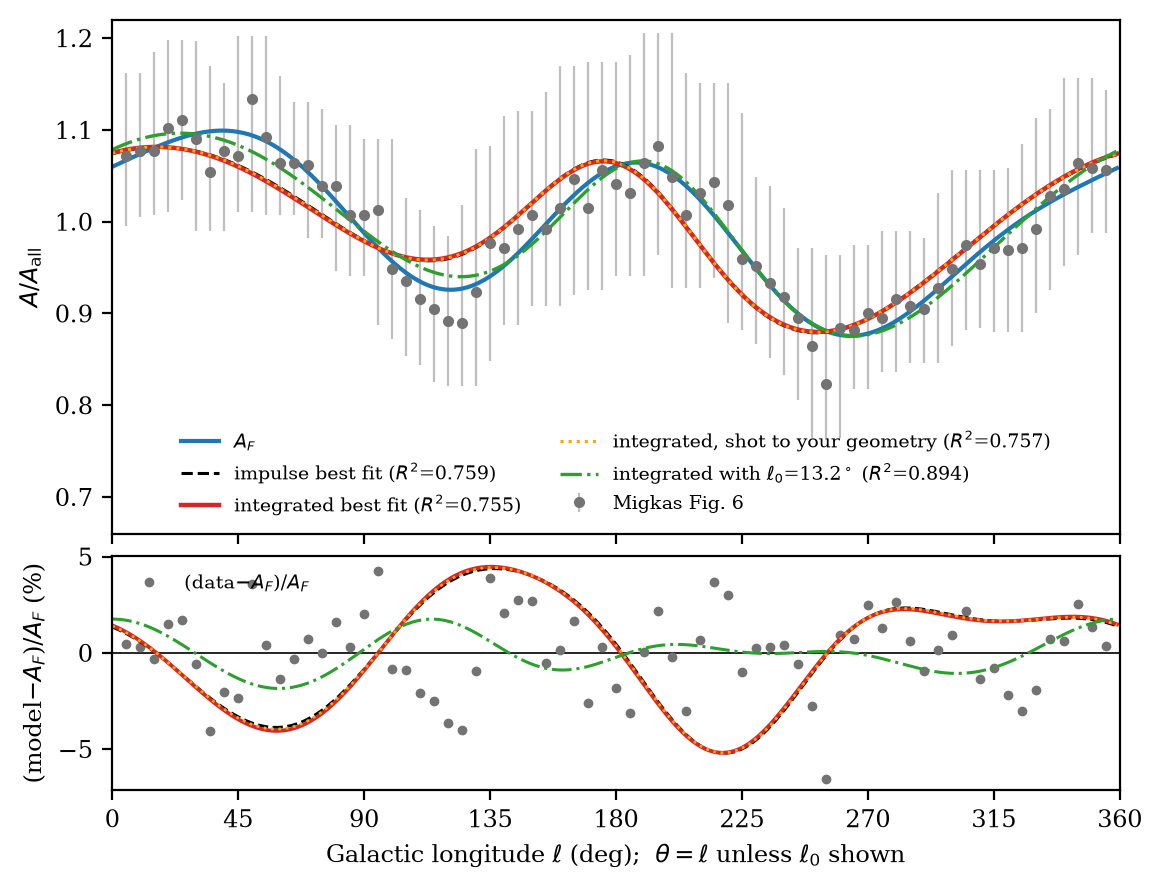
\includegraphics[width=0.86\textwidth]{integrated_bestfit.png}
\caption{Migkas points with $A_F$, the impulse best fit (dashed), and the integrated best fits: fixed profile (red), shot onto your geometry (dotted), and with the $\ell_0$ offset (dash-dot). The lower panel shows each curve and the data as a percent difference from $A_F$, $100\,(A-A_F)/A_F$.}\label{fig:best}
\end{figure}

\begin{figure}[H]\centering
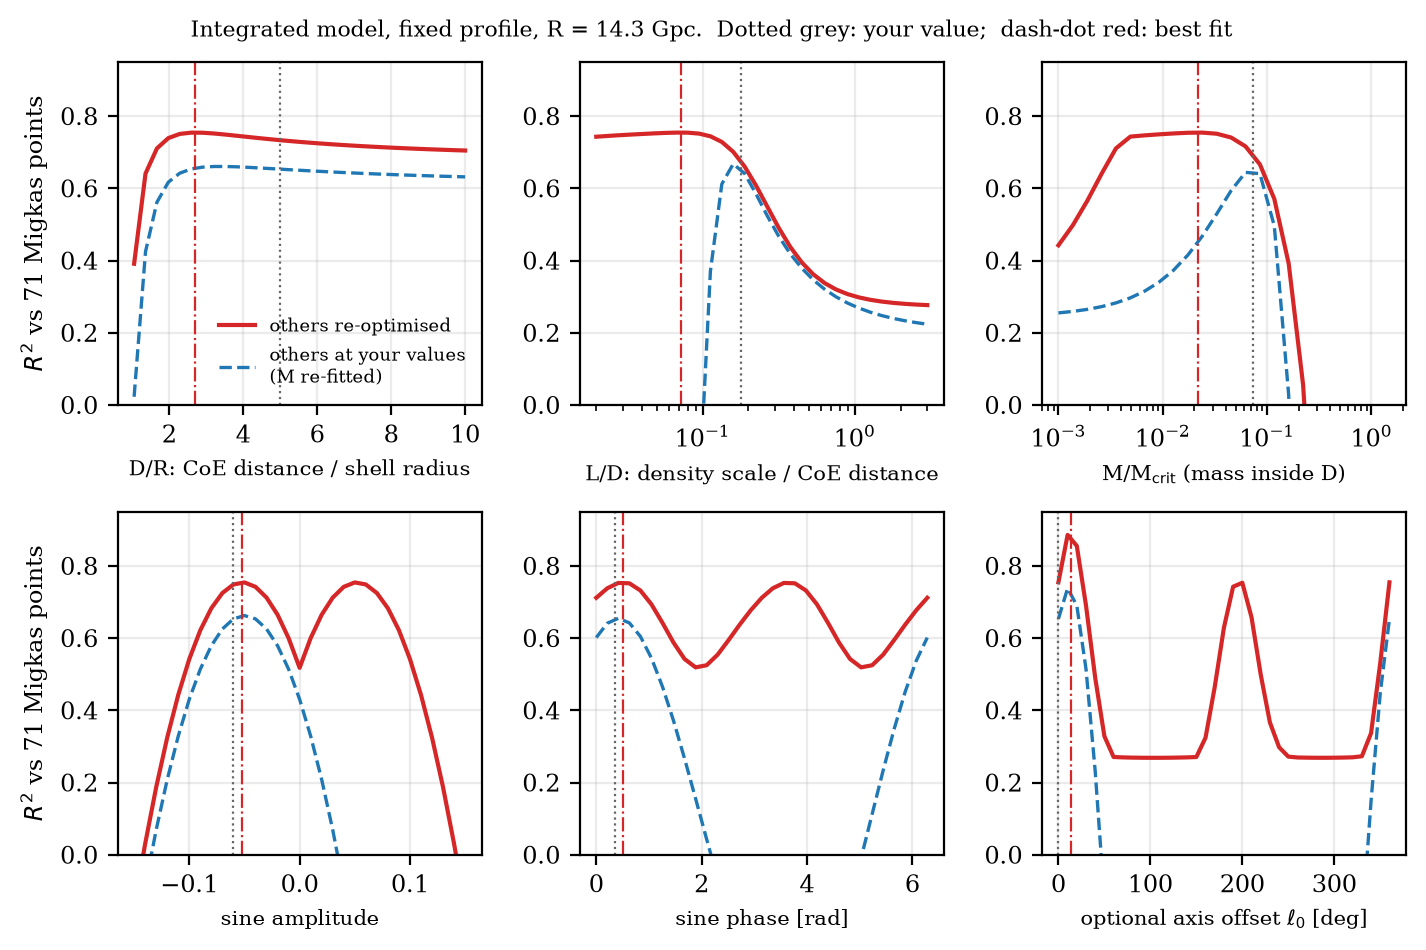
\includegraphics[width=0.9\textwidth]{integrated_profiles.png}
\caption{One-parameter scans of the integrated fixed-profile model. In the solid curves all other parameters are re-optimised. In the dashed curves the others stay at your values with $M$ re-fitted, because your literal $M$ recollapses. Curves end where particles turn around before today. Amp and $\varphi+\pi$ with $-$Amp describe the same curve, which gives the twin peaks.}\label{fig:prof}
\end{figure}

\begin{figure}[H]\centering
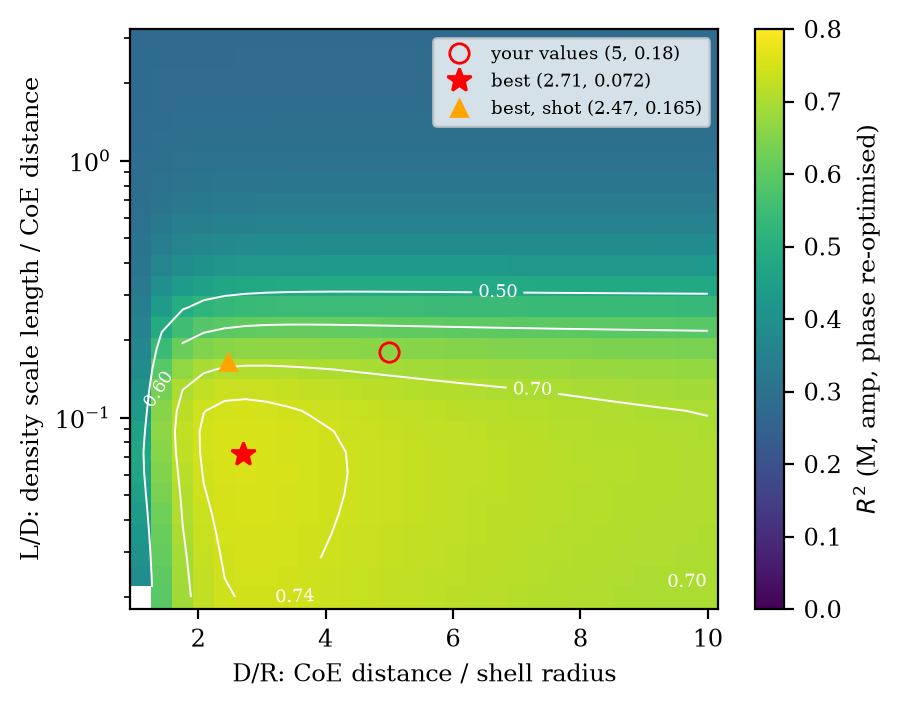
\includegraphics[width=0.5\textwidth]{integrated_DR_LD.png}
\caption{$R^2$ against the Migkas points over $D/R$ and $L/D$, with $M$, Amp and $\varphi$ re-fitted at each point, for the integrated fixed-profile model. White cells turn around before today.}\label{fig:map}
\end{figure}
\end{document}
